\documentclass{article}
\usepackage{fontspec}
\setmainfont{Times New Roman}
\usepackage{geometry}
\usepackage{CTEX}
\geometry{papersize={21cm,29.7cm}}
\geometry{left=3.18cm,right=3.18cm,top=2.54cm,bottom=2.54cm}
\usepackage{fancyhdr}
\usepackage{amsmath}
\pagestyle{fancy}
\lhead{学号:202000460020}
\rhead{姓名:苏博南}
\cfoot{\thepage}
\renewcommand{\headrulewidth}{0.4pt}
\renewcommand{\headwidth}{\textwidth}
\usepackage{tikz}
\usetikzlibrary{automata, positioning, arrows}
\usepackage{listings}
\usepackage{float}

\newtheorem{question}{题目}  
\lstset{
	basicstyle=\small\ttfamily,	% 基本样式
		keywordstyle=\color{blue}, % 关键词样式
		commentstyle=\color{gray!50!black!50},   	% 注释样式
		stringstyle=\rmfamily\slshape\color{red}, 	% 字符串样式
	backgroundcolor=\color{gray!0},     % 代码块背景颜色
	frame=leftline,						% 代码框形状
	framerule=12pt,%
		rulecolor=\color{gray!0},      % 代码框颜色
	numbers=left,				% 左侧显示行号往左靠, 还可以为right ,或none,即不加行号
		numberstyle=\footnotesize\itshape,	% 行号的样式
		firstnumber=1,
		stepnumber=1,                  	% 若设置为2,则显示行号为1,3,5
		numbersep=7pt,               	% 行号与代码之间的间距
	aboveskip=.25em, 			% 代码块边框
	showspaces=false,               	% 显示添加特定下划线的空格
	showstringspaces=false,         	% 不显示代码字符串中间的空格标记
	keepspaces=true, 					
	showtabs=false,                 	% 在字符串中显示制表符
	tabsize=2,                     		% 默认缩进2个字符
	captionpos=b,                   	% 将标题位置设置为底部
	flexiblecolumns=true, 			%
	breaklines=true,                	% 设置自动断行
	breakatwhitespace=false,        	% 设置自动中断是否只发生在空格处
	breakautoindent=true,			%
	breakindent=1em, 			%
	title=\lstname,				%
	escapeinside=``,  			% 在``里显示中文
	xleftmargin=1em,  xrightmargin=1em,     % 设定listing左右的空白
	aboveskip=1ex, belowskip=1ex,
	framextopmargin=1pt, framexbottommargin=1pt,
        abovecaptionskip=-2pt,belowcaptionskip=3pt,
	% 设定中文冲突,断行,列模式,数学环境输入,listing数字的样式
	extendedchars=false, columns=flexible, mathescape=true,
	texcl=true,
	fontadjust
}%

\begin{document}

\begin{center}
    \huge{机器学习课程实验四}\\
    \large{\today \quad 苏博南\quad 202000460020}
\end{center}

\section{二分类的Linear Discrimination Analysis}

相关原理省略,只考虑算法流程。记$x$为一$m\times n$的矩阵表示训练集合,$C_i$表示第$i$个类别,$i=1,2$。
则:
\begin{itemize}
    \item [1.] 计算平均点:$\mu_i=\frac{1}{n_i}\sum_{x\in C_i}x,i=1,2$,其中$n_i$表示类别为$C_i$的样本数量。
    \item [2.] 计算类内散度矩阵:$S_w=\sum_{i=1}^C\sum_{x\in C_i}(x-\mu_i)(x-\mu_i)^T$.
    \item [3.] 计算投影向量:$\theta^*=S_w^{-1}(\mu_1-\mu_2)$
    \item [4.] 作出每个样本点在直线$\overrightarrow{\theta^*}$上的投影。
\end{itemize}

在给出一个预测样本$x$,只需要计算$y=\theta^{*T}x$然后将$y$与$\gamma=\frac{n_1\theta^{*T}\mu_1+n_2\theta^{*T}\mu_2}{n_1+n_2}$比较,得到分类结果。

算法代码如下:
\begin{lstlisting}[language=matlab]
    blue = load("ex3Data/ex3blue.dat");
    red = load("ex3Data/ex3red.dat");

    plot(blue(:, 1), blue(:, 2), 'b*');
    hold on;
    plot(red(:, 1), red(:, 2), 'r.');
    axis([0, 10, 0, 10]);

    mu_blue = mean(blue)';
    mu_red = mean(red)';

    [m, n] = size(blue);
    S_w = zeros(n, n);
    for i = 1 : m
        S_w = S_w + (blue(i, :)' - mu_blue) * (blue(i, :)' - mu_blue)';
    end
    [m, n] = size(red);
    for i = 1 : m
        S_w = S_w + (red(i, :)' - mu_red) * (red(i, :)' - mu_red)';
    end

    theta = S_w \ (mu_blue - mu_red);

    xs = 0 : 0.1 : 10;
    ys = theta(2) / theta(1) * xs;
    plot(xs, ys, 'k-');

    for i = 1 : size(blue, 1)
        p = projects(theta, blue(i, :)');
        line([blue(i, 1), p(1)], [blue(i, 2), p(2)], 'LineStyle', '--', 'Color', 'k', 'LineWidth', 0.5);
        plot(p(1), p(2), 'b*');
    end

    for i = 1 : size(red, 1)
        p = projects(theta, red(i, :)');
        line([red(i, 1), p(1)], [red(i, 2), p(2)], 'LineStyle', '--', 'Color', 'k', 'LineWidth', 0.5);
        plot(p(1), p(2), 'r.');
    end

    function pos = projects(line, point)
        t = (point' * line) / (line' * line);
        pos = t * line;
    end
\end{lstlisting}

得到的结果如下图所示:
\begin{figure}[H]
    \centering
    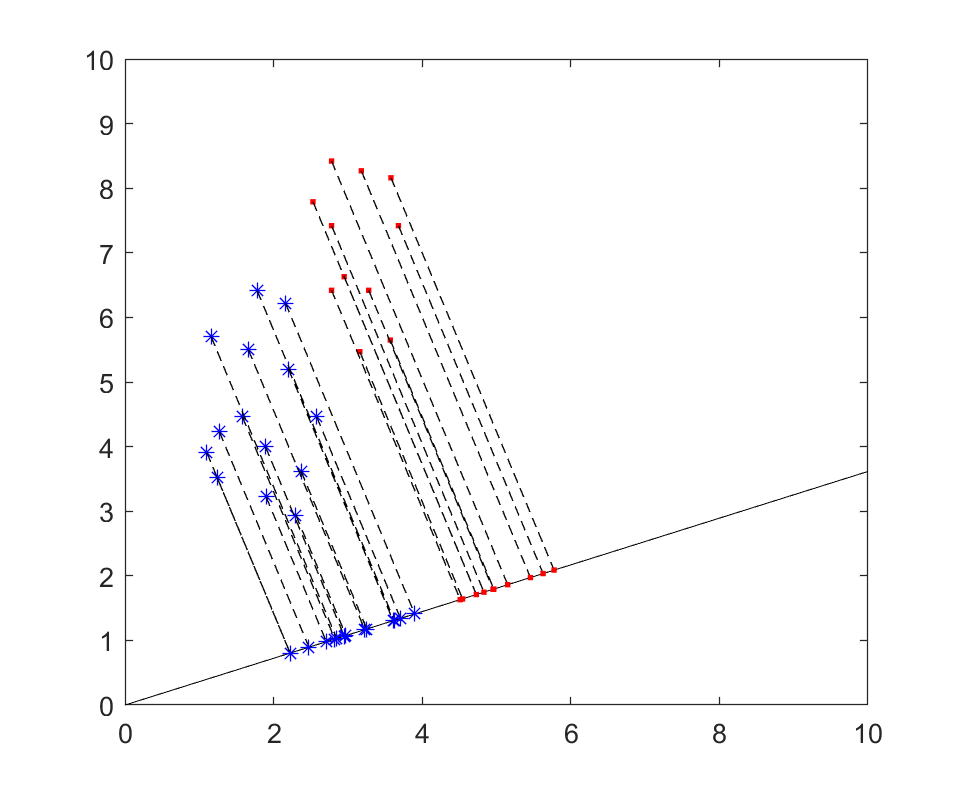
\includegraphics[width=\linewidth]{1.png}
\end{figure}

\section{多分类的LDA}

算法流程:
\begin{itemize}
    \item [1.] 计算平均点$\mu_i=\frac{1}{n_i}\sum_{x\in C_i}x$。
    \item [2.] 计算类间散度矩阵$S_b=\frac{1}{2N}\sum_{i,j=1}^C n_in_j(\mu_i-\mu_j)(\mu_i-\mu_j)^T$
    \item [3.] 计算类内散度矩阵$S_w=\sum_{i=1}^C\sum_{x\in C_i}(x-\mu_i)(x-\mu_i)^T$
    \item [4.] 选择$S_w^{-1}S_b$的前p大的特征值对应的特征向量$\{\theta_1,\theta_2,...,\theta_p\}$。
\end{itemize}

在实验中,由于样本数据维度为两维,只有两个特征值,我们选择其中大的哪一个。
算法代码如下:
\begin{lstlisting}[language=matlab]
    blue = load("ex3Data/ex3blue.dat");
    red = load("ex3Data/ex3red.dat");
    green = load("ex3Data/ex3green.dat");

    plot(blue(:, 1), blue(:, 2), 'b.');
    hold on;
    plot(red(:, 1), red(:, 2), 'r.');
    plot(green(:, 1), green(:, 2), 'g.');

    axis([0, 10, 0, 10]);

    mu_blue = mean(blue)';
    mu_red = mean(red)';
    mu_green = mean(green)';

    mu = (sum(blue) + sum(red) + sum(green)) / (size(blue, 1) + size(red, 1) + size(green, 1));
    mu = mu';

    S_b = size(blue, 1) * (mu_blue - mu) * (mu_blue - mu)' + size(red, 1) * (mu_red - mu) * (mu_red - mu)' + size(green, 1) * (mu_green - mu) * (mu_green - mu)';

    S_w = zeros(2, 2);
    for i = 1 : size(blue, 1)
        S_w = S_w + (blue(i, :) - mu_blue) * (blue(i, :) - mu_blue)';
    end
    for i = 1 : size(red, 1)
        S_w = S_w + (red(i, :) - mu_red) * (red(i, :) - mu_red)';
    end
    for i = 1 : size(green, 1)
        S_w = S_w + (green(i, :) - mu_green) * (green(i, :) - mu_green)';
    end

    S = S_w \ S_b;
    [V, D] = eig(S);
    [mx, i] = max(diag(D));
    theta = V(:, i);

    xs = 0 : 0.1 : 10;
    ys = theta(2) / theta(1) * xs;
    plot(xs, ys, 'k-');

    for i = 1 : size(blue, 1)
        p = projects(theta, blue(i, :)');
        line([blue(i, 1), p(1)], [blue(i, 2), p(2)], 'LineStyle', '--', 'Color', 'k', 'LineWidth', 0.5);
        plot(p(1), p(2), 'b*');
    end

    for i = 1 : size(red, 1)
        p = projects(theta, red(i, :)');
        line([red(i, 1), p(1)], [red(i, 2), p(2)], 'LineStyle', '--', 'Color', 'k', 'LineWidth', 0.5);
        plot(p(1), p(2), 'r.');
    end

    for i = 1 : size(green, 1)
        p = projects(theta, green(i, :)');
        line([green(i, 1), p(1)], [green(i, 2), p(2)], 'LineStyle', '--', 'Color', 'k', 'LineWidth', 0.5);
        plot(p(1), p(2), 'g.');
    end

    function pos = projects(line, point)
        t = (point' * line) / (line' * line);
        pos = t * line;
    endblue = load("ex3Data/ex3blue.dat");
    red = load("ex3Data/ex3red.dat");
    green = load("ex3Data/ex3green.dat");

    plot(blue(:, 1), blue(:, 2), 'b.');
    hold on;
    plot(red(:, 1), red(:, 2), 'r.');
    plot(green(:, 1), green(:, 2), 'g.');

    axis([0, 10, 0, 10]);

    mu_blue = mean(blue)';
    mu_red = mean(red)';
    mu_green = mean(green)';

    mu = (sum(blue) + sum(red) + sum(green)) / (size(blue, 1) + size(red, 1) + size(green, 1));
    mu = mu';

    S_b = size(blue, 1) * (mu_blue - mu) * (mu_blue - mu)' + size(red, 1) * (mu_red - mu) * (mu_red - mu)' + size(green, 1) * (mu_green - mu) * (mu_green - mu)';

    S_w = zeros(2, 2);
    for i = 1 : size(blue, 1)
        S_w = S_w + (blue(i, :) - mu_blue) * (blue(i, :) - mu_blue)';
    end
    for i = 1 : size(red, 1)
        S_w = S_w + (red(i, :) - mu_red) * (red(i, :) - mu_red)';
    end
    for i = 1 : size(green, 1)
        S_w = S_w + (green(i, :) - mu_green) * (green(i, :) - mu_green)';
    end

    S = S_w \ S_b;
    [V, D] = eig(S);
    [mx, i] = max(diag(D));
    theta = V(:, i);

    xs = 0 : 0.1 : 10;
    ys = theta(2) / theta(1) * xs;
    plot(xs, ys, 'k-');

    for i = 1 : size(blue, 1)
        p = projects(theta, blue(i, :)');
        line([blue(i, 1), p(1)], [blue(i, 2), p(2)], 'LineStyle', '--', 'Color', 'k', 'LineWidth', 0.5);
        plot(p(1), p(2), 'b*');
    end

    for i = 1 : size(red, 1)
        p = projects(theta, red(i, :)');
        line([red(i, 1), p(1)], [red(i, 2), p(2)], 'LineStyle', '--', 'Color', 'k', 'LineWidth', 0.5);
        plot(p(1), p(2), 'r.');
    end

    for i = 1 : size(green, 1)
        p = projects(theta, green(i, :)');
        line([green(i, 1), p(1)], [green(i, 2), p(2)], 'LineStyle', '--', 'Color', 'k', 'LineWidth', 0.5);
        plot(p(1), p(2), 'g.');
    end

    function pos = projects(line, point)
        t = (point' * line) / (line' * line);
        pos = t * line;
    end
\end{lstlisting}

得到的结果如下图所示:
\begin{figure}[H]
    \centering
    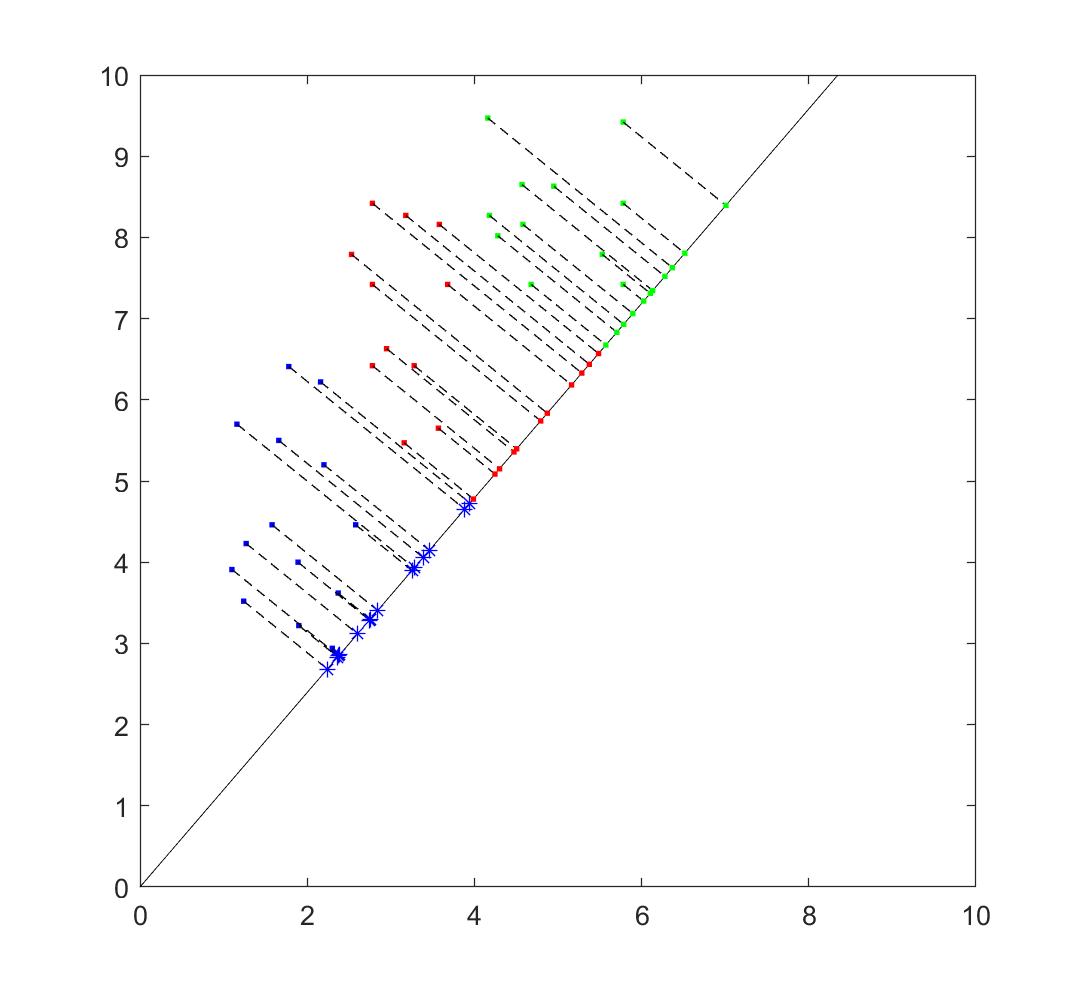
\includegraphics[width=0.7\textwidth]{2.png}
\end{figure}
\end{document}